\section*{Question 3}

In the last section we concluded that the Euclidean metric outperformed the
Manhattan metric for the kNN classifier in the provided datasets. For k=30, the best
performer of question 1, the Manhattan metric had a generalized error of $0.165$, worse
than the generalized error for the Euclidean metric ($0.160$).

We know evaluate the traning and testing error of the kNN classifier with
Euclidean metric versus it's model capacity, modeled as capacity=$1/k$.
For that, we trained the model from k=$1$ to k=$100$ (inclusive), generating
the capacity between 0.1 and 1. The results are shown in figure \ref{fig:Q3}.

The most notable feature of the error rate evolution, is the training error going to
0 at high model capacity, even thought the testing/generalized error is higher than
for lower model capacities. This is a visualization of the {\bf overfitting}
problem that can affect hihg capacity model, where the training error fails to
represent the generalization error due to high variance.

Reflecting the discussion of question 1, the low capacity models are also unable to generalize well,
but due to excessive bias, resulting in higher testing error than models with average capacity. The
lowest training error is shown by the doted line, and it happens for k=30, suggesting that the best
kNN classifier from the options evaluated until now is indeed the kNN for k=30 and the {\it Euclidean}
metric.


\renewcommand{\thefigure}{12}
\begin{figure}[h!]
    \centering
    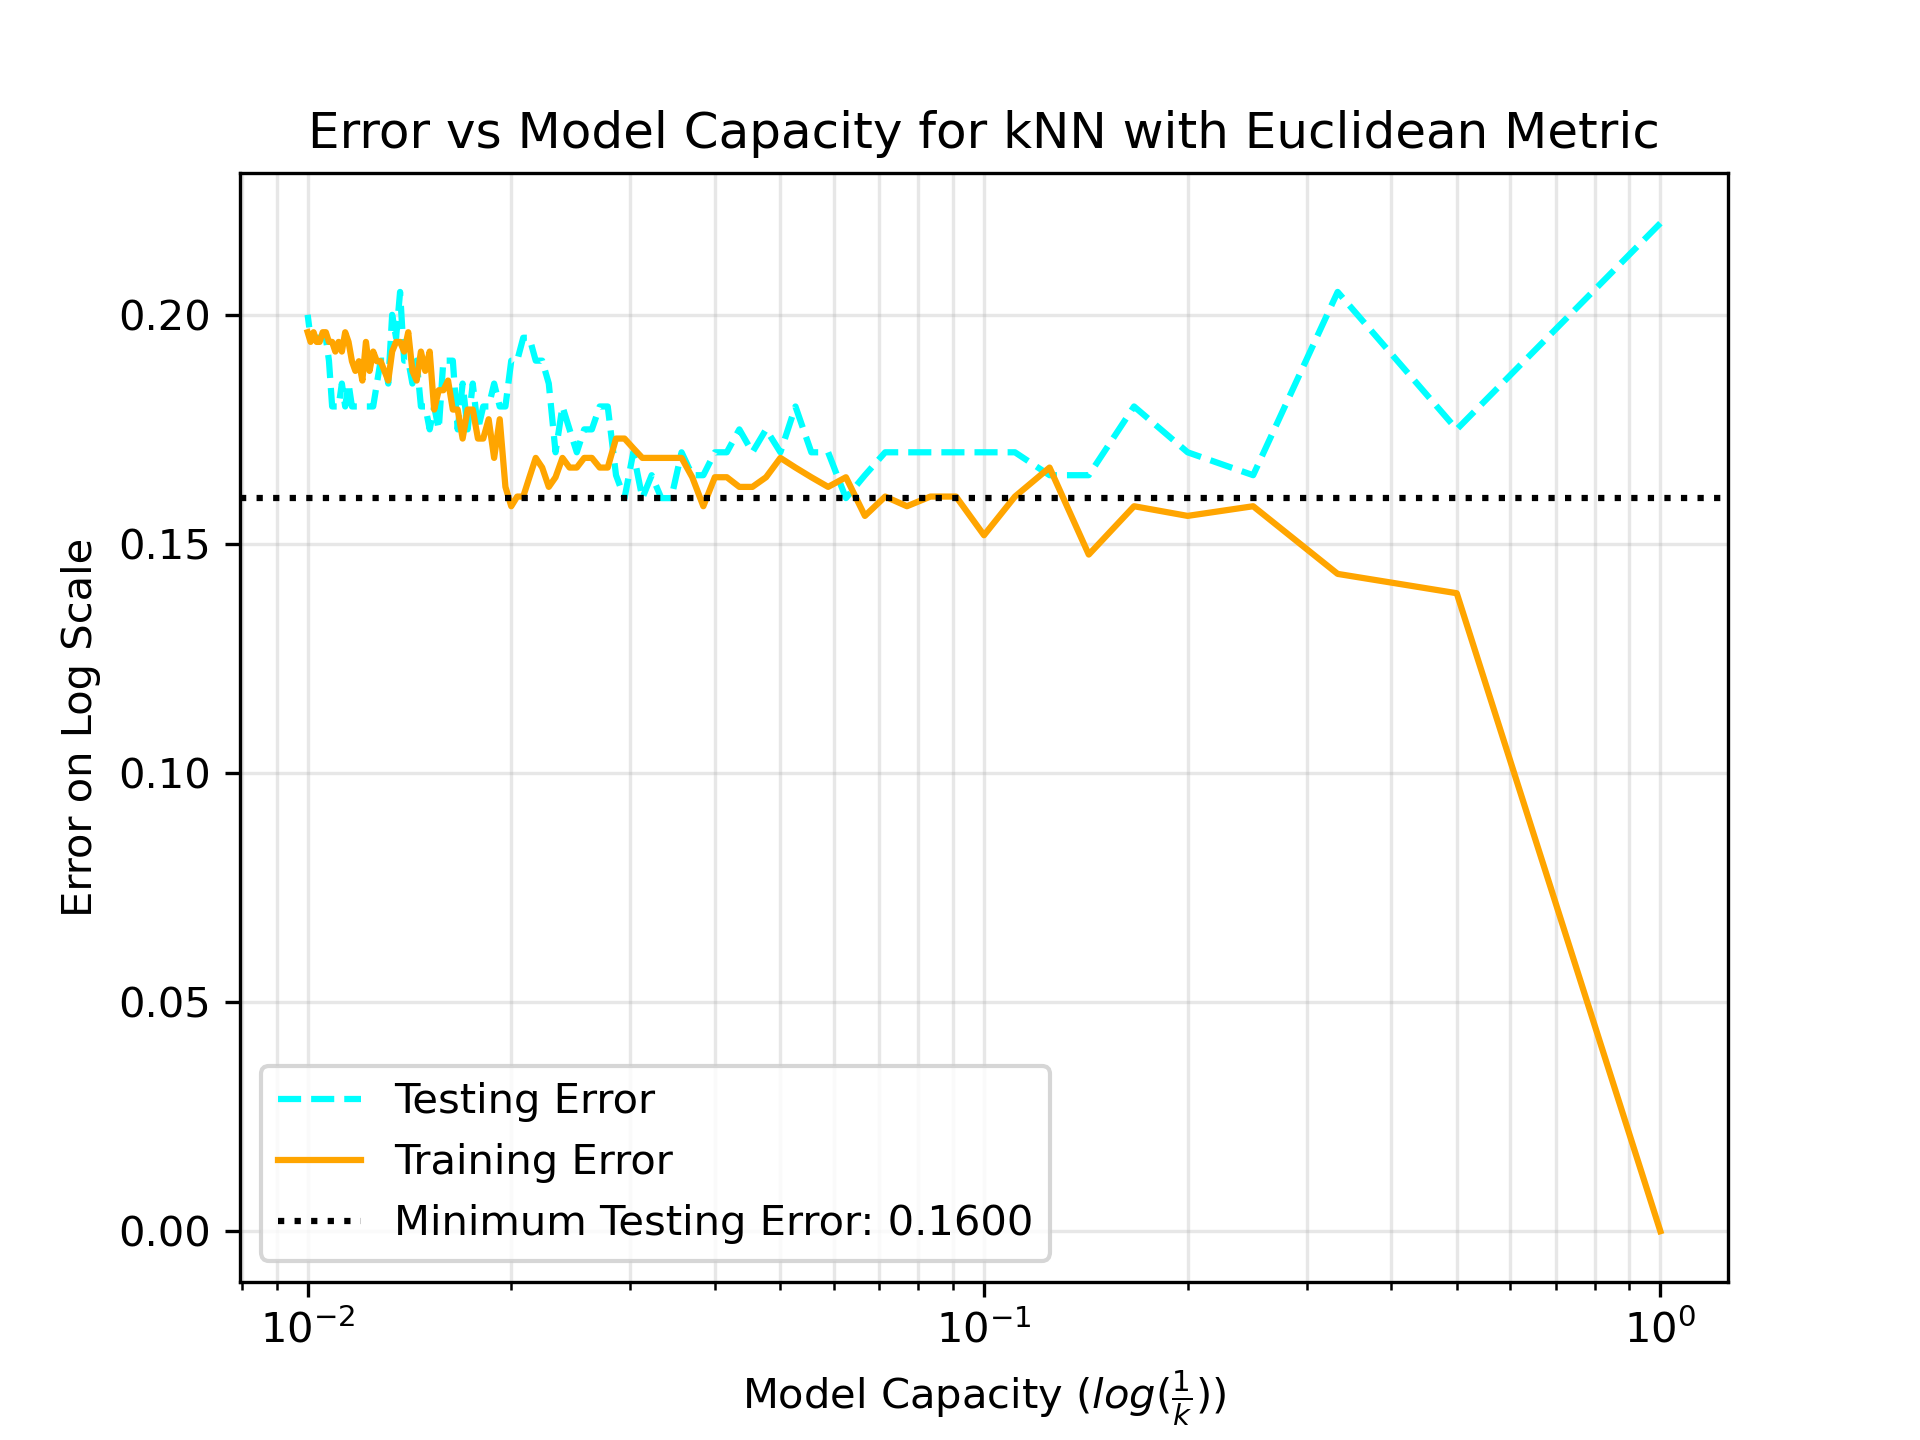
\includegraphics[width=\singleWidth]{Graphs/Q3.png}
    \caption{Error rate for kNN classifier with Euclidean Metric versus model capacity ($1\k$), where k is the number of neighbors. The capacity is shown in logscale}
    \label{fig:Q3}
\end{figure}



